%!TEX root=main.tex
\section{Diagnosing a Trend} \label{sec:data}
Before the LHC became operational in 2010, there were strong expectations for new physics and accordingly there existed a whole landscape of BSM models. 
The Higgs boson was discovered in 2012, but none of the searches for new physics turned up anything significant enough to indicate BSM physics.
Analyses are increasingly constraining the existing BSM models, and designing experimental searches based on model-specific predictions seems less and less fruitful. 
Physicists are thus increasingly turning to alternative methods for searching for new physics, they are using simplified models and so-called model-independent approaches, among them EFTs.
This trend away from model-guided searches and towards model-independent approaches can already be documented with simple bibliographic means.
As an example, Figure~1 shows the results of a keyword search that compares some of the most popular BSM models in the Higgs sector with model-independent approach of the Higgs EFT and precision measurements.  
The papers plotted employ supersymmetric Higgs models, composite Higgs models, extended Higgs sector models that are non-supersymmetric, and the Higgs EFT approach. 

The search was conducted on the popular physics preprint archive, arxiv.org.
Specifically, it was conducted on the phenomenology archive HEP-PH, the most relevant to models in high-energy physics.
We have shown in previous publications that such keyword searches provide a good first look at the dynamics of particle physics models and that the corresponding trends can be confirmed by expert interviews.\footnote{For a full description of the methods used, see [reference omitted].}
The main reason such figures provide a reasonable first look is that the mentioned preprint archives are the main scientific venue for particle physicists.
Additionally, ArXiv.org features an automatic keyword tagging system.
This system provides us with a simple method of gauging some of the trends in particle physics by seeing how the numbers of papers with different keywords change over time.\footnote{The keywords used were the following. For EFT: find k "Higgs" and (k "effective field theory" or k "precision measurement"). For SUSY: find (k "supersymmetry"or k "minimal supersymmetric standard model" or k "MSSM") and k "Higgs". For Composite Higgs: find (k "technicolor" or k “Higgs particle: composite" or k "Higgs particle: Goldstone particle" or k "pNGB" or k "top: condensation" or k "little Higgs model" or k "dynamical symmetry breaking") and k "Higgs" and not (k "supersymmetry" or k "minimal supersymmetric standard model" or k "effective field theory"). For Non-SUSY extended Higgs: find (k "Higgs particle: doublet: 2" or k "2HDM" or k "Higgs particle: triplet" or k "Higgs particle: doublet: 3" or k "Higgs particle: charged particle") and not (k "supersymmetry*" or k "minimal supersymmetric standard model" or k "effective field theory") }
The keyword searches were conducted in such a way as to minimize overlap between the terms by specifying for instance that the composite Higgs papers include neither supersymmetric models nor an EFT approach. 
\begin{figure}
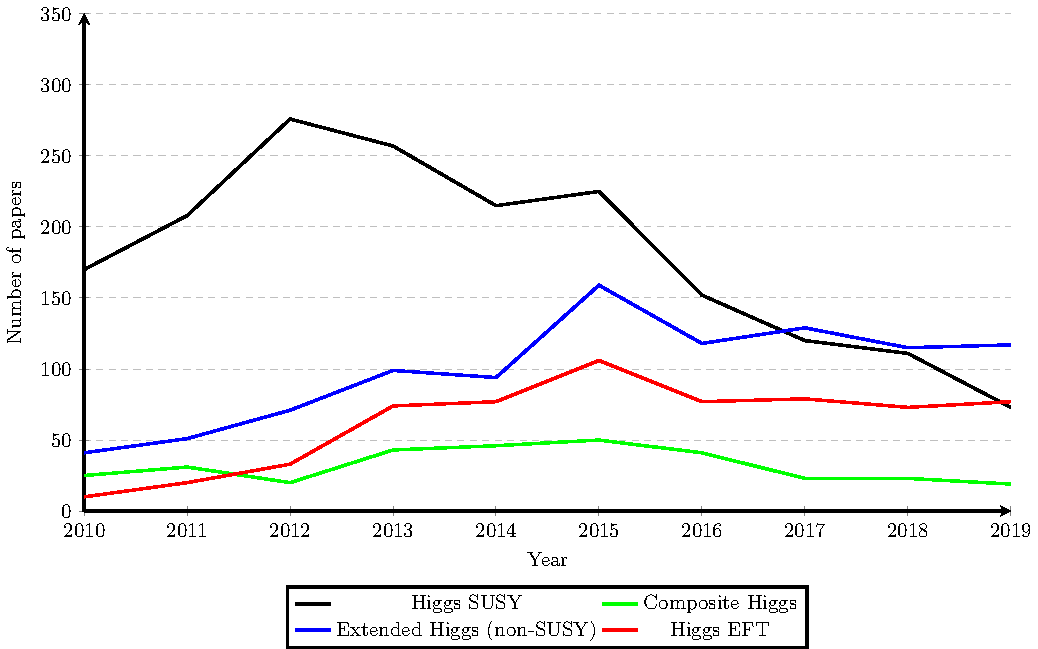
\includegraphics[width=\textwidth]{susyeft_2107}
\caption{The number of papers per year for the most popular BSM models in the Higgs sector and the the Higgs EFT.} 
\label{fig:lineplot}
\end{figure}

\begin{figure}
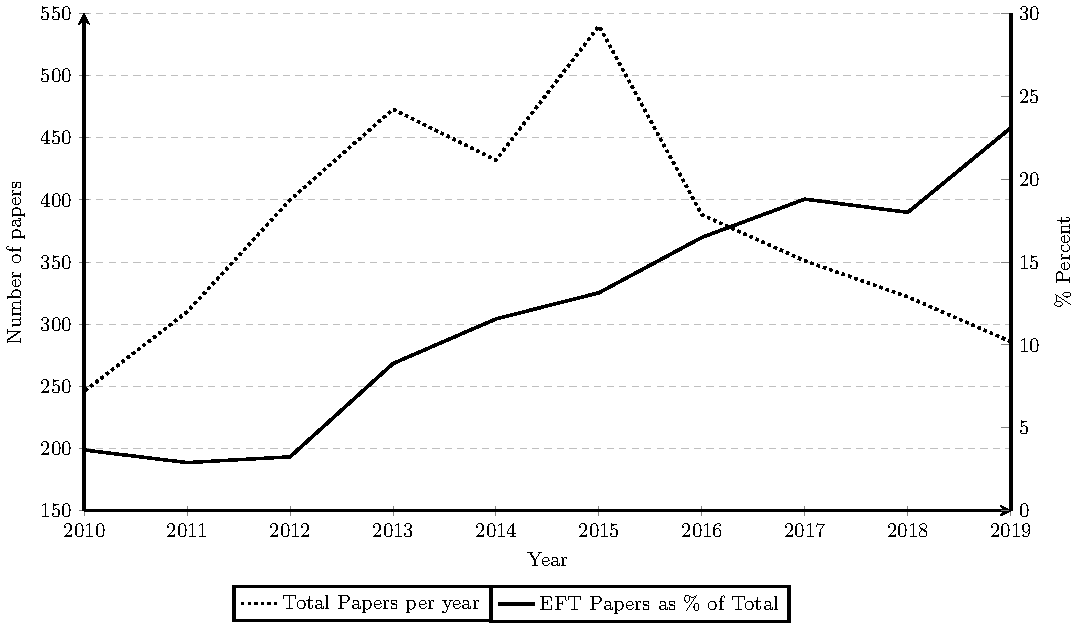
\includegraphics[width=\textwidth]{percenttotal_eft_2107}
\caption{The total number of papers from the most popular models of BSM in the Higgs sector (sum from left plot) against the number of papers on Higgs EFT as a percentage of that total.}
\label{fig:percent}
\end{figure}


One can see in Fig.~\ref{fig:lineplot} a flurry of model building up to and past the Higgs discovery, lasting until 2015. 
Since then, there has been an overall decrease in the number of papers on Higgs models, in particular a strong decrease in supersymmetric models. 
The number of non-supersymmetrically extended Higgs models is growing, but more slowly than the number of papers of supersymmetric models is declining, hence the decreasing total. 
It is also not a single model, but captures many different minimal extensions.
What is of most interest to us in this paper is that the number of papers on the Higgs EFT approach climbs steadily. 
As a result, while the total number of papers is on a downtrend, there is an strongly increasing percentage of these papers that employs the Higgs EFT approach. 
The increase plotted in Fig.~\ref{fig:percent} is quite dramatic.
Of course, the Higgs sector is only a part of the research of high energy physics, but this is indicative of the trend in the field at large. 
We take this data as a jumping off point that shows that there is a trend that is worth the attention of philosophers.
We also take this to indicate that there is a real distinction in physics practice between the model-based and model-independent approaches.  
Part of our aim in the paper is to characterise this distinction and investigate how one should understand this trend in the context of the contemporary debates on the nature of models, theories, and EFTs.
